%%
%% This is file `sample-sigconf.tex',
%% generated with the docstrip utility.
%%
%% The original source files were:
%%
%% samples.dtx  (with options: `sigconf')
%% 
%% IMPORTANT NOTICE:
%% 
%% For the copyright see the source file.
%% 
%% Any modified versions of this file must be renamed
%% with new filenames distinct from sample-sigconf.tex.
%% 
%% For distribution of the original source see the terms
%% for copying and modification in the file samples.dtx.
%% 
%% This generated file may be distributed as long as the
%% original source files, as listed above, are part of the
%% same distribution. (The sources need not necessarily be
%% in the same archive or directory.)
%%
%% The first command in your LaTeX source must be the \documentclass command.
\documentclass[sigconf]{acmart}

%%
%% \BibTeX command to typeset BibTeX logo in the docs
\AtBeginDocument{%
  \providecommand\BibTeX{{%
    \normalfont B\kern-0.5em{\scshape i\kern-0.25em b}\kern-0.8em\TeX}}}

%% Rights management information.  This information is sent to you
%% when you complete the rights form.  These commands have SAMPLE
%% values in them; it is your responsibility as an author to replace
%% the commands and values with those provided to you when you
%% complete the rights form.

%%
%% Submission ID.
%% Use this when submitting an article to a sponsored event. You'll
%% receive a unique submission ID from the organizers
%% of the event, and this ID should be used as the parameter to this command.
%%\acmSubmissionID{123-A56-BU3}

%%
%% The majority of ACM publications use numbered citations and
%% references.  The command \citestyle{authoryear} switches to the
%% "author year" style.
%%
%% If you are preparing content for an event
%% sponsored by ACM SIGGRAPH, you must use the "author year" style of
%% citations and references.
%% Uncommenting
%% the next command will enable that style.
%%\citestyle{acmauthoryear}


\usepackage{array}
\newcommand{\head}[2]{\multicolumn{1}{>{\centering\arraybackslash}p{#1}}{\textbf{#2}}}

\usepackage{listings}



%%
%% end of the preamble, start of the body of the document source.
\begin{document}

%%
%% The "title" command has an optional parameter,
%% allowing the author to define a "short title" to be used in page headers.
\title{Meltdown: Reading Kernel Memory from User Space}

%%
%% The "author" command and its associated commands are used to define
%% the authors and their affiliations.
%% Of note is the shared affiliation of the first two authors, and the
%% "authornote" and "authornotemark" commands
%% used to denote shared contribution to the research.
\author{Enrik Doçi}
%%\authornote{Both authors contributed equally to this research.}
\email{enrik.doci@b-tu.de}
\orcid{1234-5678-9012}
\affiliation{%
  \institution{Brandenburg Technical University}
  \streetaddress{Universitatsstrasse 1}
  \city{Cottbus}
  \state{Germany}
  \postcode{03046}
}

%%
%% By default, the full list of authors will be used in the page
%% headers. Often, this list is too long, and will overlap
%% other information printed in the page headers. This command allows
%% the author to define a more concise list
%% of authors' names for this purpose.
\renewcommand{\shortauthors}{Enrik Doçi}

%%
%% The abstract is a short summary of the work to be presented in the
%% article.
\begin{abstract}
  A clear and well-documented \LaTeX\ document is presented as an
  article formatted for publication by ACM in a conference proceedings
  or journal publication. Based on the ``acmart'' document class, this
  article presents and explains many of the common variations, as well
  as many of the formatting elements an author may use in the
  preparation of the documentation of their work.
\end{abstract}

%%
%% The code below is generated by the tool at http://dl.acm.org/ccs.cfm.
%% Please copy and paste the code instead of the example below.
%%


%%
%% Keywords. The author(s) should pick words that accurately describe
%% the work being presented. Separate the keywords with commas.
\keywords{out-of-order execution, side-channel attack, transient instruction, + others}


%%
%% This command processes the author and affiliation and title
%% information and builds the first part of the formatted document.
\maketitle

\section{Introduction}

Content to be added later

\section{Background}
To properly understand how Meltdown works, more specifically the steps to bypass memory isolation by taking advantage of out-of-order execution and further use timing differences in cache memory to create a covert channel, it is important to understand the purpose of each component used during this attack, and how they operate. This section is focused on the basics of memory hierarchy (caching and virtual memory) and an overview of CPU architecture to further understand out-of-order execution. 
\subsection{Memory Hierarchy}
\subsubsection{Caching}
The need for fast memory that could keep up with the CPU frequency is limited by the high cost per byte these high-performance memories come with.
To address this issue, extremely fast registers are placed inside the CPU, small but fast memory is assigned to the CPU, a slightly slower but random-based accessable memory is assigned to the running applications, and the secondary memory for storing data at rest. 

The memory close to the CPU, called a cache, takes advantage of {\itshape spatial locality} (data to be processed tend to be close to the data already being processed) and {\itshape temporal locality} (processed data tends to be requested multiple times during execution).

A typical architecture consists of 3 levels of caches, with two being private per core and the third one being shared. For efficiency, data is moved in {\itshape blocks} (or lines) which contain a fixed size of words. Placing the blocks in cache can be made via different schemes, such as {\itshape set associative} (each block has a pre-determined position in cache), {\itshape n-way set associative} (each block can be placed in one of n possible positions in cache) or {\itshape fully associative} (the block can be placed anywhere in cache).

The memory and speed of a typical modern desktop computer \cite{Hennessy:2017:CAS:3207796} tends to be as follows :

\begin{table}[h]
  \label{tab:freq}
  \begin{tabular}{p{0.66cm}|p{0.75cm}p{0.75cm}p{0.75cm}p{0.75cm}p{1cm}p{1cm}}
     & \textbf{CPU Reg.} & \textbf{L1 cache} & \textbf{L2 Cache} & \textbf{L3 Cache} & \textbf{Main Mem.} & \textbf{Secon. Mem.}\\
     \hline
    Size & 2000 Bytes & 64 KB & 256 KB & 8-32 MB & 8-64 GB & 256 GB - 2 TB\\
    \hline
    Speed & 300 ps & 1 ns & 3-10 ns & 10-20 ns & 50-100 ns & 50-100 $\mu$s\\
  %\bottomrule
\end{tabular}
\caption{Memory hierarchy for a Desktop Computer}
\end{table}

\subsubsection{Virtual Memory}
Each process runs within its own address space, so there is a need to share the limited main memory between all running processes. The method used to achieve this is through {\itshape virtual memory}; the physical memory is divided into blocks called pages, and allocated to any process in need for memory. The processor issues virtual memory addresses for memory operations, which are mapped to physical ones using page translation tables. The translation table is held inside a CPU register, and it is per-process only; the operating system updates them for every process being executed. 

In order for processes not to access the blocks of other processes, protection schemes have to apply. Translation tables have privilege checks that are 

\subsection{CPU Architecture and out-of-order Execution}

The CPU architectures affected by the attack mentioned in this paper have all a microarchitecture that is pipelined, super-scalar, out-of-order and with speculative execution. This section will further explain each of these methods used to perform instruction-level parallelism (ILP).

{\itshape Pipelining} is a technique which allows multiple instructions to overlap during execution, each using different resources oft he processor. Standartization of instruction in execution phases such as fetch, decode, execute, memory access and write-back, which do not have hardware dependencies between them. 

{\itshape Superscalar} processors can execute more than one instruction during a clock cycle. This is not the same as multi-core processor, but rather having multiple execution resources inside the CPU, for example ALUs. 

{\itshape Speculative execution} means that the compiler or the processor tries to guess the outcome of an instruction, thus removing it as a dependency in the execution path of other instructions. Since out focus is the hardware architecture, the main speculative execution on a processor ist hat of branch predicition, explained below. 

{\itshape Out-of-order execution} makes it possible for instructions to continue execution the moment all the required resources are available, even when the previous one is blocked and waitting for other operations to be completed. This is not to be confused with speculative execution below; in out-of-order execution all the instructions are correctly executed and no assumptions are made. Still, all the execution results stay at an microarchitecture state till all prior instructions are commited. 

\begin{figure}[h]
  \centering
  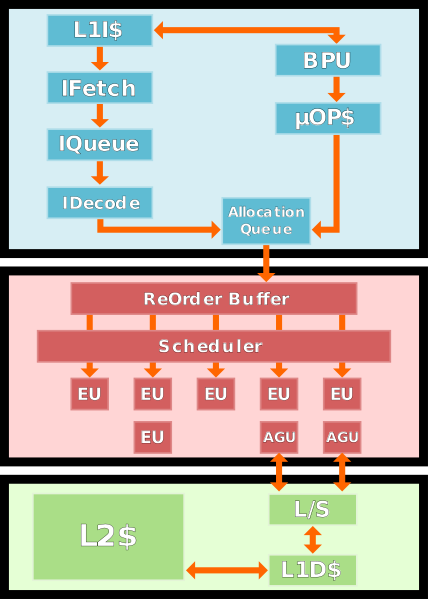
\includegraphics[width=\linewidth]{skylake_simple_diagram}
  \caption{Simplified design of a Skylake Core.}  
  \Description{The 1907 Franklin Model D roadster.}
\end{figure}

\footnote{ for detailed picture, choose skylake\_block\_diagram [Public domain maybe? check!!!], via (). }

The first step to achieve out-of-order execution is to solve data hazards (data dependencises from previous instructions), such as read-after-write, write-after-read and write-after-write (RAW, WAR, WAW). Normally, even in a pipelined datapath, the output from a previous instruction would be available only after the last phase, memory writeback. Tomasulo \cite{Cohen07} suggested the use of a unified reservation station that would make the outputs available the moment they were ready, and not having to wait for it to be stored and re-read using common data bus (CDB), that connects all execution units with each-other. 

In the front-end, instructions are decoded into micro-ops ($\mu$-ops), and are sent into the IDQ ($\mu$-op queue). Breaking every instruction into $\mu$-ops makes it possible for any procesor to execute commands without the need of modifying the instruction set. They are later sent to the back-end (execution engine) where the logic of out-of-order is implemented. They are later forwarded to the scheduler, which decides on which execution unit u-ops should be send depending on their specific task. 

BPU (Branch Prediction Unit) decides on branch instructions which block of code will be executed, before knowing for sure the correct flow of the execution. This prediction is usually a trade secret, and only the manufacterer knows the algorithm used, but the main ways to predict a path are : ---content here--- Instructions on the path that is going to be executed, start executing immediately as long as they don‘t have any dependencies. Upon realizing that the prediction was incorrect, the reorder buffer is rolled-back to a correct state (flushed) and the unified reservation station is re-initialized. This way, unauthorized instructions are executed and can change the microarchitectural state, but the change will not be reflected on the architecture state. 

\subsection{Flush+Reload}

Flush+Reload\cite{Knuth97} is a side-channel attack technique with minimal noise induction, that has been used to implement in practice Meltdown attacks. This attack exploits a weakness on Intel X86 processors, where access to memory lines in shared pages can be monitored, and used to leak informations from processes. It targets the L3 cache, thus the attack can be performed even on other execution cores. 

\section{Meltdown}

The main idea of meltdown is to throw an unhandled exception, which will cause the operating system to take control of the execution flow and handle the exeption. This means that the control flow will execute in kernel mode. Till now, nothing out of the ordinary happens, but due to out-of-order execution, the next few instructions being executed, now will run on kernel space and not user space. These instructions will not be retired, thus not saving the microarchitectural changes and the results of the executed instructions.

To have access to kernel data, a simple move instruction can be performed, causing the byte referenced in the memory to be fetched and stored in a register, and also cached . While not much can be done to retrieve the data from te register since it will not be commited, the cached values will continue to stay on.

The following machine code instructions can be easily used to give the basic concept of the attack, while removing the complexity of a real world example. 
\begin{lstlisting}
; rcx = a protected kernel memory address
; rbx = address of a large array in user space
mov al, byte [rcx]         
shl rax, 0xc
mov rbx, qword [rbx + rax]
\end{lstlisting}

The move instruction reads the byte at address where the register rcx points to, and copies the value to register al. Since this address falls under the kernel space, an exeption will be thrown, and the execution will jump to the exception handler. In this case the exception will be a page fault, and the operating system will flush the re

\section{Real-World attacks}

Text here

\section{Countermeasures and Mitigation}

Text here 

\section{Related Works}

Exploitation can be observed during multiple steps of ILP. In the front-end this can happen during speculation via branch prediction (BPU), albeit difficult to exploit in the wild due to the mechanics of dynamic branch prediction not being publicly known. Exploitations can further be performed during dynamic scheduling (BPU \& IFU) and speculative execution (IDQ).

In the back-end exploitations can be observed during the register renaming (allocate/rename/retire unit), superscalar and out-of-order (scheduler) and in-order commit (retirement).

\subsection{Spectre}

While Meltdown makes use of the out-of-order execution to read and leak kernel memory that under normal execution they should not have, Spectre uses speculative execution property of branch prediction (conditional and indirect branches) to read arbitrary memory. Before BPU realizes the branch was wrongly predicted, some instructions are already speculatively executed, and through a side channel the confidential information is sent from a microarchitectural state to an architectural one. 

Unlike Meltdown, Spectre works on a wide range of processors, including most ARM and AMD models and not just Intel and some ARM. Also, KAISER mechanism used to mitigate Meltdown, doesn't protect against Spectre. 

\subsection{ZombieLoad}

ZombieLoad is another Meltdown-like attack that benefits from fault-driven transient instruction execution. This exploitation is performed on the fill-buffer using faulty Load instructions that have to be re-issued internally but don't become architecturaly visible. The values accessed by these Load instructions are those of recent registers belonging to previous memory operations from the current or a sibling hyperthread, unlike Meltdown that has to use explicit address-based selectors. Protection against ZombieLoad can be achived only by disabling hyperthreading. 

\subsection{Cache Side-channel Attacks}

While at 2.3 Flush+Reload was used to transmit the data from the microarchitectural state to the attacker process, any other cache side-channel attack can be used. Such side-channel attacks are as below : \cite{8686667}

\subsubsection{Evict+Time}

Text here

\subsubsection{Prime+Probe}

\subsubsection{Evict+Time}

\newpage
%%
%% The next two lines define the bibliography style to be used, and
%% the bibliography file.
\bibliographystyle{ACM-Reference-Format}
\bibliography{sample-base}

%%
%% If your work has an appendix, this is the place to put it.
\appendix

\end{document}
\endinput
%%
%% End of file `sample-sigconf.tex'.
